
\documentclass[12pt, a4paper]{article}
\usepackage{../../../myconfig} % Gọi file cấu hình từ ngoài gốc vào

% ==========================================
% BẮT ĐẦU NỘI DUNG TÀI LIỆU
% ==========================================
\begin{document}

% Truyền 3 tham số: {Nhãn cam} {Chữ to chính giữa} {Chữ ở góc phải Header}
\titlebox{Chủ đề: Tích phân}{Ứng dung tích phân tính diện hình phẳng thực tế}{Nguyên hàm - Tích phân: Ứng dụng}

\questionShortAnswer{0}{1}{Một vòng xuyến ở ngã tư thành phố Tam Điệp có dạng hình tròn đường kính \( AB = 6m \). Công ty cây xanh thiết kế phần trồng hoa giấy ở giữa hai đường parabol có trục đối xứng vuông góc với đường kính \( AB \) tại tâm của hình tròn và cắt \( AB \) tại điểm \( C, C' \) thỏa mãn \( BC = 2m \) (phần tô đậm). Phần còn lại của vòng xuyến thiết kế trồng hoa có các chi phí để trồng hoa giấy và hoa cúc lần lượt là 200 000 đồng/m² và 100 000 đồng/m². Hỏi chi phí để trang trí vòng xuyến theo thiết kế là bao nhiêu nghìn đồng (kết quả làm tròn đến hàng đơn vị)?

\begin{center}
\begin{tikzpicture}[scale=1.2, >=latex]
    \fill[pattern=north east lines, pattern color=black!80]
        plot[domain=-1:1, samples=100] (\x, {-2*\x*\x + 2}) --
        plot[domain=1:-1, samples=100] (\x, {2*\x*\x - 2}) -- cycle;

    % 2. Vẽ đường tròn bao ngoài (bán kính R = 2)
    \draw[thick] (0,0) circle (2);

    % 3. Vẽ đường kính AB
    \draw[thick] (-2,0) -- (2,0);

    % 4. Vẽ parabol úp (phía trên)
    \draw[thick, samples=100, domain=-1:1] 
        plot (\x, {-2*\x*\x + 2});

    % 5. Vẽ parabol ngửa (phía dưới)
    \draw[thick, samples=100, domain=-1:1] 
        plot (\x, {2*\x*\x - 2});

    % 6. Nhãn các điểm
    \node[left] at (-2,0) {\small $A$};
    \node[right] at (2,0) {\small $B$};
    \node[below left] at (-1,0) {\small $C'$};
    \node[below right] at (1,0) {\small $C$};
\end{tikzpicture}
\end{center}
}

\questionShortAnswer{0}{2}{Một công ty đang thiết kế một bảng quảng cáo hình chữ nhật \(ABCD\) có kích thước \(AB=15m\) và \(AD=10m\). Phần trung tâm của bảng sẽ được in nội dung quảng cáo, được mô tả là phần tô đậm (xem hình minh họa). Hai đường cong trong hình là một phần của đồ thị hàm số \(y=\frac{ax+b}{cx+d}\), đường tiệm cận đứng và tiệm cận ngang của đồ thị hàm số này đều cách điểm \(A\) một khoảng bằng \(5m\). Đồ thị giao với cạnh \(AB\) tại điểm \(E\) thỏa mãn \(\frac{AE}{AB}=\frac{8}{15}\). Diện tích phần in nội dung quảng cáo là bao nhiêu mét vuông (kết quả làm tròn đến hàng phần đơn vị)?

\begin{center}
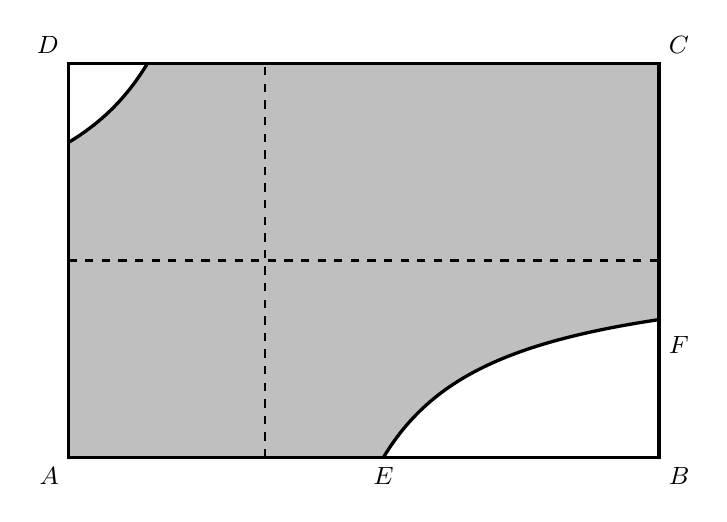
\begin{tikzpicture}[scale=0.5, >=latex]
   \begin{scope}
        % Tô nền xám ABCD (0,0) đến (15,10)
        \fill[gray!50] (0,0) rectangle (15,10);
          \fill[white] 
            plot[domain=0:2, samples=100] (\x, {5 - 15/(\x - 5)}) -- (0,10) -- cycle;
        \fill[white] 
            (8,0) -- plot[domain=8:15, samples=100] (\x, {5 - 15/(\x - 5)}) -- (15,0) -- cycle;
    \end{scope}

    % 2. Khung hình chữ nhật ABCD
    \draw[very thick] (0,0) rectangle (15,10);

    % 3. Vẽ hai nhánh đồ thị hàm phân thức
    \draw[very thick, samples=100, domain=0:2] 
        plot (\x, {5 - 15/(\x - 5)});
    \draw[very thick, samples=100, domain=8:15] 
        plot (\x, {5 - 15/(\x - 5)});

    % 4. Các đường tiệm cận nét đứt (cách A một khoảng 5m -> x = 5 và y = 5)
    \draw[thick, dashed] (5,0) -- (5,10);
    \draw[thick, dashed] (0,5) -- (15,5);

    % 5. Đánh dấu các đỉnh và điểm
    \node[below left] at (0,0) {\small $A$};
    \node[below right] at (15,0) {\small $B$};
    \node[above right] at (15,10) {\small $C$};
    \node[above left] at (0,10) {\small $D$};
    
    \node[below] at (8,0) {\small $E$};
    \node[right] at (15, 2.85) {\small $F$};
\end{tikzpicture}
\end{center}
}

\questionShortAnswer{0}{3}{Mẫu gạch lát nền nhà được thiết kế có dạng hình vuông cạnh 6dm, bốn góc viên gạch màu trắng, phần ở giữa sẫm màu (hình vẽ). Đường viền của phần sẫm màu bao gồm bốn đoạn thẳng nằm trên các cạnh hình vuông và bốn đường cong có tính chất: tích khoảng cách từ một điểm bất kì thuộc đường cong đó đến hai trục đối xứng (khác hai đường chéo) của viền gạch bằng \(3dm^2\). Tính diện tích phần sẫm màu (đơn vị: decimét vuông) (kết quả làm tròn đến hàng phần mười)?

\begin{center}
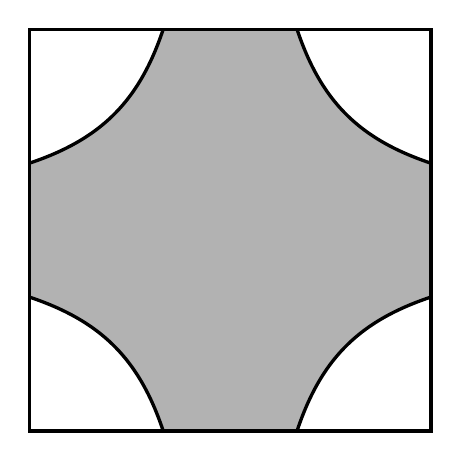
\begin{tikzpicture}[scale=0.85, >=latex]
    % 1. Tô màu xám phần sẫm màu ở giữa
    % Hình vuông [-3,3] x [-3,3], 4 góc trắng bị cắt bởi y = 3/x
    \begin{scope}
        % Tô màu xám toàn bộ hình vuông
        \fill[gray!60] (-3,-3) rectangle (3,3);

        % Trừ góc 1 (trên - phải)
        \fill[white] (1,3) -- plot[domain=1:3, samples=100] (\x, {3/\x}) -- (3,1) -- (3,3) -- cycle;
        % Trừ góc 2 (trên - trái)
        \fill[white] (-1,3) -- plot[domain=-1:-3, samples=100] (\x, {-3/\x}) -- (-3,1) -- (-3,3) -- cycle;
        % Trừ góc 3 (dưới - trái)
        \fill[white] (-1,-3) -- plot[domain=-1:-3, samples=100] (\x, {3/\x}) -- (-3,-1) -- (-3,-3) -- cycle;
        % Trừ góc 4 (dưới - phải)
        \fill[white] (1,-3) -- plot[domain=1:3, samples=100] (\x, {-3/\x}) -- (3,-1) -- (3,-3) -- cycle;
    \end{scope}

    % 2. Khung hình vuông bao ngoài
    \draw[very thick] (-3,-3) rectangle (3,3);

    % 3. Vẽ 4 đường cong hyperbol ở 4 góc
    \draw[very thick, samples=100, domain=1:3] plot (\x, {3/\x});
    \draw[very thick, samples=100, domain=-3:-1] plot (\x, {-3/\x});
    \draw[very thick, samples=100, domain=-3:-1] plot (\x, {3/\x});
    \draw[very thick, samples=100, domain=1:3] plot (\x, {-3/\x});
\end{tikzpicture}
\end{center}
}

\questionShortAnswer{0}{4}{Bác An lên kế hoạch làm một cái biển quảng cáo phẳng, có thiết kế là phần được tô màu đậm trong hình vẽ bên dưới. Đường cong \( (P) \) là một parabol có đỉnh là điểm \( F \), có trục đối xứng là \( FH \) và đi qua các điểm \( A, B \). Tứ giác \( ABCD \) là hình chữ nhật, \( AB = 6m, BC = 2m, EF = 5m, FH = 1m \). Bác An kí hợp đồng với công ty X với đơn giá là 1,2 triệu đồng/1 \( m^2 \). Hỏi số tiền mà bác An phải trả sau khi làm xong cái biển quảng cáo là bao nhiêu triệu đồng?
\begin{center}
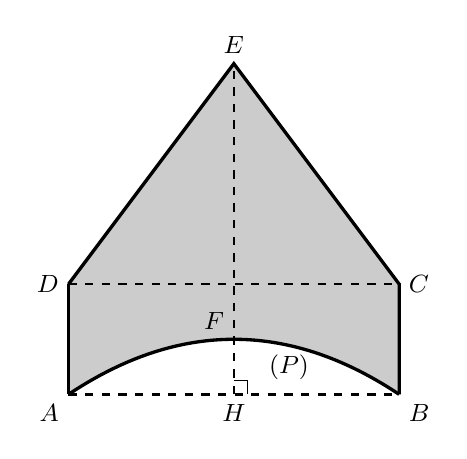
\begin{tikzpicture}[scale=0.7, >=latex]
    % 1. Tô màu xám phần biển quảng cáo
    \begin{scope}
        \fill[gray!40] 
            (-3,2) -- (0,6) -- (3,2) -- (3,0) -- 
            plot[domain=3:-3, samples=100] (\x, {-1/9*\x*\x + 1}) -- (-3,2) -- cycle;
    \end{scope}

    % 2. Đường nét đứt hỗ trợ
    \draw[thick, dashed] (-3,0) -- (3,0); % Đoạn AB
    \draw[thick, dashed] (-3,2) -- (3,2); % Đoạn CD
    \draw[thick, dashed] (0,0) -- (0,6);  % Trục EH qua F, H

    % 3. Khung viền phần tô đậm
    \draw[very thick] (-3,2) -- (0,6) -- (3,2) -- (3,0);
    \draw[very thick] (-3,2) -- (-3,0);
    \draw[very thick, samples=100, domain=-3:3] plot (\x, {-1/9*\x*\x + 1});

    % 4. Đánh dấu các góc vuông tại H
    \draw (0,0.25) -- (0.25,0.25) -- (0.25,0);

    % 5. Đánh dấu các tên điểm
    \node[below left] at (-3,0) {\small $A$};
    \node[below right] at (3,0) {\small $B$};
    \node[right] at (3,2) {\small $C$};
    \node[left] at (-3,2) {\small $D$};
    \node[above] at (0,6) {\small $E$};
    \node[above left] at (0,1) {\small $F$};
    \node[below] at (0,0) {\small $H$};
    \node[below] at (1, 0.9) {\small $(P)$};
\end{tikzpicture}
\end{center}
}

\questionShortAnswer{0}{5}{Viên gạch men dùng để lát nền nhà là một hình vuông có cạnh bằng 80 cm (xem hình bên dưới). Mỗi viên gạch có 4 bông hoa, mỗi bông hoa gồm 4 cánh hoa. Mỗi cánh hoa (phần màu xanh) là phần giao nhau của hai hình tròn có cùng bán kính và khoảng cách giữa hai tâm là \( 20\sqrt{2} \, \text{cm} \). Ước tính ở công đoạn trắng men, phần màu xanh có chi phí 50 nghìn đồng trên một mét vuông, còn phần màu trắng có chi phí 30 nghìn đồng trên một mét vuông. Tính chi phí (đơn vị: tỉ đồng) của công đoạn trắng men này, khi cơ sở dự định sản xuất 100 000 viên gạch như thế (kết quả làm tròn đến hàng phần trăm).
\begin{center}
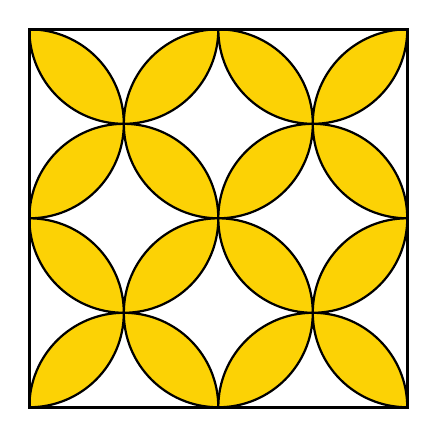
\begin{tikzpicture}[scale=0.06]
    % Khai báo màu xanh Teal cho phần nền
    \definecolor{tealgreen}{RGB}{0,128,128}

    % 1. Tô nền màu xanh cho toàn bộ viên gạch 80x80
    \fill [white] (0,0) rectangle (80,80);

   
    \fill[yellow!70!orange, draw=black, thick] (20,60) arc (0:90:20) arc (180:360:20) arc (90:270:20) arc (0:180:20) arc (-90:0:20) ;
    
    \fill[yellow!70!orange, draw=black, thick] (60,60) arc (0:90:20) arc (180:360:20) arc (90:270:20) arc (0:180:20) arc (-90:0:20) ;

    \fill[yellow!70!orange, draw=black, thick] (20,20) arc (0:90:20) arc (180:360:20) arc (90:270:20) arc (0:180:20) arc (-90:0:20) ;

    \fill[yellow!70!orange, draw=black, thick] (60,20) arc (0:90:20) arc (180:360:20) arc (90:270:20) arc (0:180:20) arc (-90:0:20) ;
   

    % 3. Viền khung viên gạch hình vuông 80x80
    \draw[very thick] (0,0) rectangle (80,80);

   
\end{tikzpicture}
\end{center}
}



\questionShortAnswer{0}{7}{Một tấm kính làm mặt bàn \( (H_1) \) có hình dáng tam giác đều với 3 đỉnh được làm cong \( (H_2) \). Biết cạnh tấm kính tam giác ban đầu bằng \( 12dm \). Để cắt góc đẹp thì người ta dùng đường Parabol  
\((P): y = -\frac{\sqrt{3}}{4}x^2 + 5\sqrt{3} \, (H_3)\)
có hai nhánh tiếp xúc với hai cạnh của tam giác.
\begin{figure}[htbp]
    \centering
    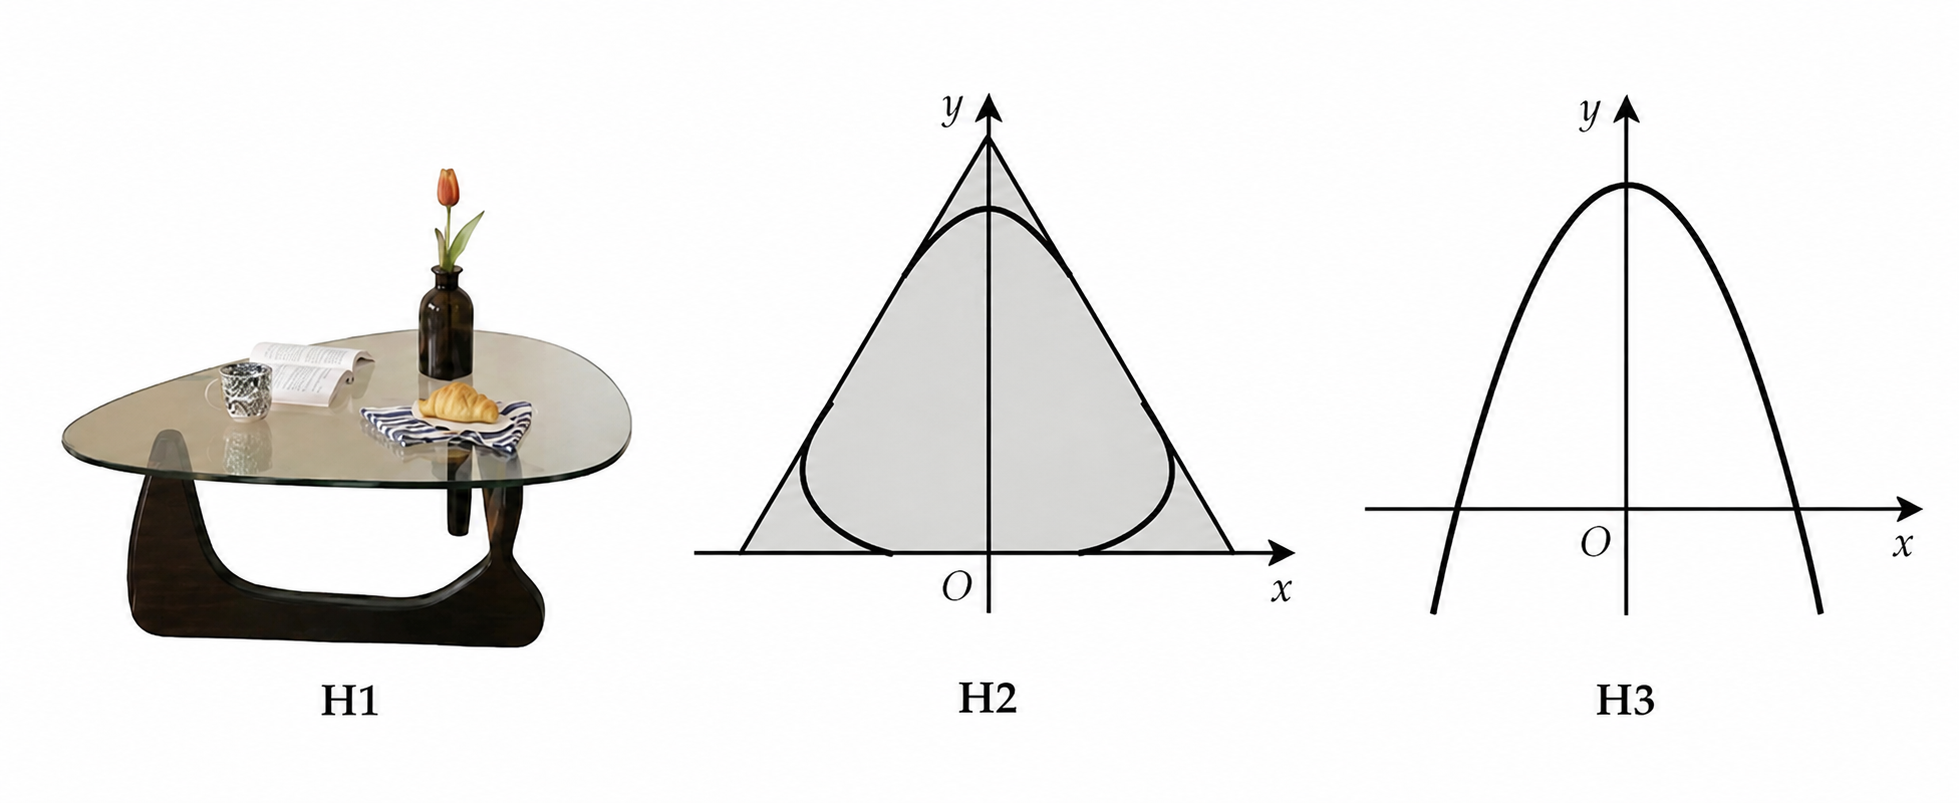
\includegraphics[width=0.4\textwidth]{../images/ban.png}
\end{figure}
Biết diện tích mặt kính là \( a\sqrt{b} \, (dm^2) \), (với \( a \) là số nguyên dương và \( b \) là số nguyên tố). Tính \( a+b \).
}


\questionTrueFalse{0}{8}{Một nhóm các kỹ sư muốn xây dựng một cây cầu vòm dàn thép với giá đỡ dưới bằng thép cao cấp có hình dáng là một đường cong Parabol nối từ 2 cột trụ A và B nằm bên dưới cây cầu, biết hai cột trụ cách nhau 400 m, khoảng cách từ trụ A đến cây cầu là 50 m và AB song song với mặt đường. Gắn hệ trục tọa độ Oxy vào cây cầu với đơn vị trục tọa độ là 10 m. Giá đỡ dưới bằng thép là đường cong Parabol tạo với 2 trục tọa độ các hình phẳng có diện tích \( S_1, S_2, S_3 \) như hình vẽ bên dưới, biết rằng \( S_2 - 2S_1 = 100 \).
\begin{figure}[htbp]
    \centering
    \includegraphics[width=0.4\textwidth]{../images/cau.png}
\end{figure}
}{
    \textbf{a)} & Đồ thị Parabol đi qua điểm có tọa độ \( (0; -5) \).
    & \textcolor{amberorange}{$\bigcirc$} & \textcolor{amberorange}{$\bigcirc$} \\ \hline
    
    \textbf{b)} & \( S_1 = S_3 \).
    & \textcolor{amberorange}{$\bigcirc$} & \textcolor{amberorange}{$\bigcirc$} \\ \hline
    
    \textbf{c)} & Hoành độ của đỉnh parabol là 20.
    & \textcolor{amberorange}{$\bigcirc$} & \textcolor{amberorange}{$\bigcirc$} \\ \hline
    
    \textbf{d)} & Điểm cao nhất của giá đỡ dưới bằng thép cao cấp cách mặt đường cây cầu 6,25 m.
    & \textcolor{amberorange}{$\bigcirc$} & \textcolor{amberorange}{$\bigcirc$} \\
}

\questionTrueFalse{0}{9}{Thành nhà Hồ nằm trên địa phận huyện Vĩnh Lộc, tỉnh Thanh Hóa được UNESCO công nhận là di sản văn hóa thế giới vào ngày 27/6/2011. Thành có bốn cổng xây bằng đá ở bốn phía Nam-Bắc-Tây-Đông (Tiền-Hậu-Tả-Hữu), trong đó phía Nam gồm 3 cửa (như hình bên), mỗi phía còn lại chỉ có một cửa, các cửa thành được xây kiểu vòm cuốn.  

Trong một buổi trải nghiệm, một nhóm học sinh thực nghiệm đo đạc cửa chính giữa của cổng phía Nam để tính diện tích phần cửa gỗ và thu được các kết quả sau: Bề rộng của cửa dưới mặt đất là 5,82m, hai bên mép cửa (coi như vuông góc với mặt đất) có độ cao 2,25m. Vòm cửa cong theo dáng của một Parabol có đỉnh là đỉnh cửa. Chiều cao từ mặt đất đến mặt trên cửa thành là 9,5m, khoảng cách từ đỉnh cửa đến mặt trên của thành là 3,75m. Nhóm học sinh chọn hệ trục tọa độ Oxy sao cho gốc tọa độ là điểm chính giữa đoạn thẳng nối hai chân cửa, trục Ox đi qua hai chân cửa, tia Oy hướng lên trên và đi qua đỉnh cửa, đơn vị trên mỗi trục tọa độ là 1 mét.  
\begin{figure}[htbp]
    \centering
    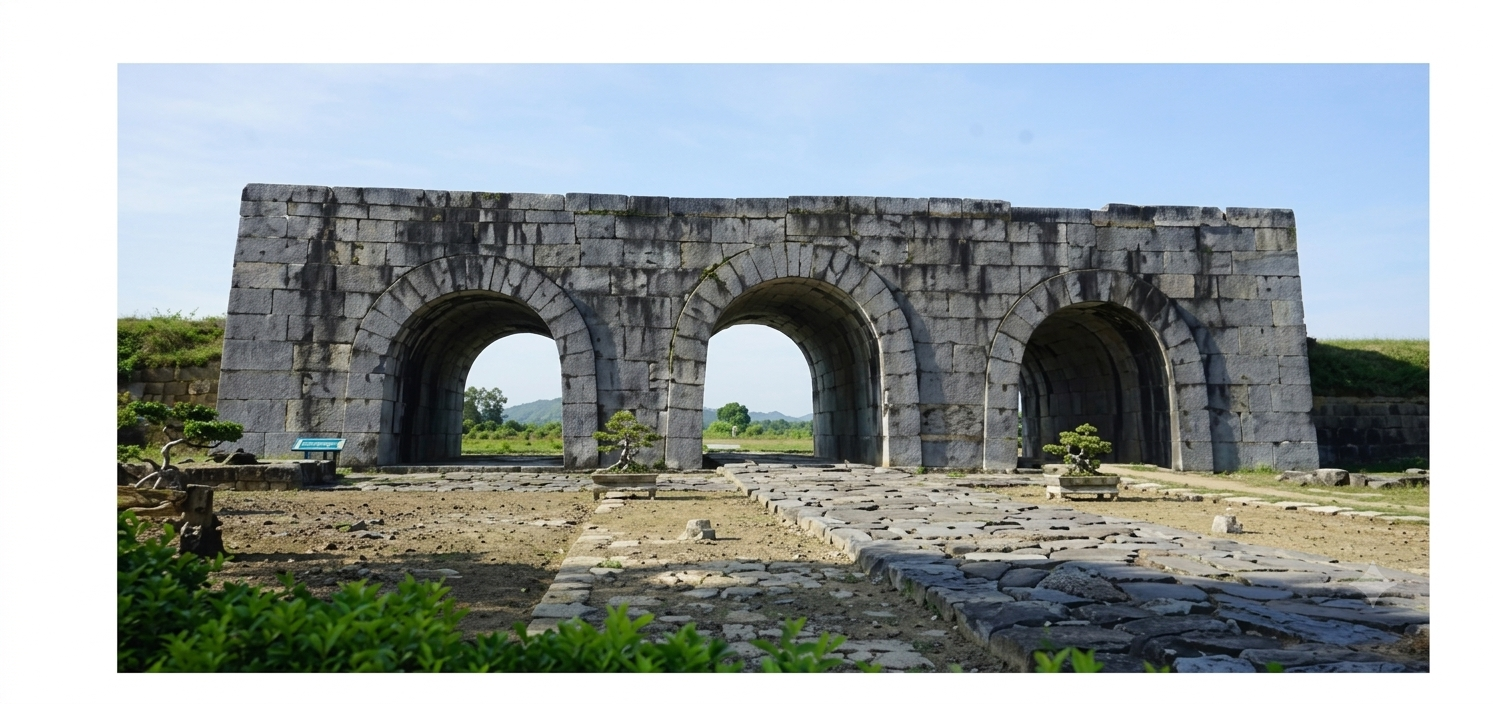
\includegraphics[width=0.4\textwidth]{../images/Thanh.png}
\end{figure}
}{
    \textbf{a)} & Chiều cao từ mặt đất đến đỉnh cửa là 5,75m.
    & \textcolor{amberorange}{$\bigcirc$} & \textcolor{amberorange}{$\bigcirc$} \\ \hline
    
    \textbf{b)} & Với hệ trục tọa độ Oxy đã chọn, đỉnh cửa là điểm \( I(0; 3,75) \).
    & \textcolor{amberorange}{$\bigcirc$} & \textcolor{amberorange}{$\bigcirc$} \\ \hline
    
    \textbf{c)} & Với hệ trục tọa độ Oxy đã chọn, vòm cửa là một phần của đồ thị hàm số  
    \(y = \dfrac{-7}{8,52}x^2 + 5,75.\)
    & \textcolor{amberorange}{$\bigcirc$} & \textcolor{amberorange}{$\bigcirc$} \\ \hline
    
    \textbf{d)} & Trước đây, ở mỗi cửa có cánh cửa làm bằng gỗ, khi khép lại thì cửa được đóng kín. Diện tích cửa gỗ của cửa chính giữa là 26,68 \( m^2 \) (kết quả làm tròn đến hàng phần trăm của đơn vị \( m^2 \)).
    & \textcolor{amberorange}{$\bigcirc$} & \textcolor{amberorange}{$\bigcirc$} \\
}

\questionTrueFalse{0}{10}{Một nhà sản xuất dự kiến xây dựng sân khấu cho một concept âm nhạc trên một mảnh đất hình chữ nhật có kích thước là \( 20m \times 10m \). Nhà sản xuất mô phỏng sân khấu thông qua bản vẽ trên hệ trục Oxy như hình vẽ. Vẽ hai parabol có đỉnh \( I_1, I_2 \) có cùng hoành độ, trong đó parabol đỉnh \( I_1 \) tiếp xúc với cạnh ngắn của hình chữ nhật. Vị trí giao nhau của hai parabol là \( A \) và \( B \) cùng với hai đỉnh \( I_1, I_2 \) tạo thành hình thoi có độ dài hai đường chéo là \( I_1I_2 = 16m \) và \( AB = 8m \) (tham khảo hình vẽ). Trên thực tế, khu vực màu đen là khu vực thiết kế dành cho khán giả, màu xám là khu vực sân khấu và màu trắng là khu vực hậu trường.  

Chi phí để xây dựng khu vực sân khấu, hậu trường, khán đài lần lượt là 2 triệu đồng, 200 nghìn đồng và 400 nghìn đồng mỗi mét vuông.  

Gắn hệ trục tọa độ sao cho \( O \) trùng với giao điểm \( AB \) và \( I_1I_2 \), \( OB \) thuộc tia \( Ox \) và \( OI_1 \) thuộc tia \( Oy \).

\begin{center}
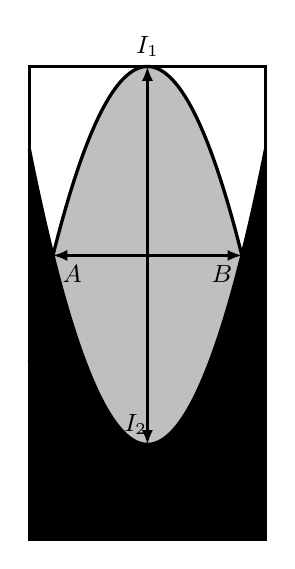
\begin{tikzpicture}[scale=0.3, >=latex]
    % 1. Tô màu các khu vực
    \begin{scope}
        % Khung mảnh đất 20x10 (-5 đến 5, -12 đến 8)
        % Tô nền màu đen cho Khán đài (dưới P2)
        % \fill[black] (-5,-12) rectangle (5,8);

        % Tô màu trắng cho Hậu trường (ngoài P1 & P2, phía trên)
        \fill[black] (-5,-12) -- plot[domain=-5:5, samples=100] (\x, {0.5*\x*\x -8}) -- (5,-12) -- cycle;
        

        % Tô màu xám cho Sân khấu (giới hạn giữa P1 và P2)
        \fill[gray!50] 
            plot[domain=-4:4, samples=100] (\x, {-0.5*\x*\x + 8}) -- 
            plot[domain=4:-4, samples=100] (\x, {0.5*\x*\x - 8}) -- cycle;
    \end{scope}

    % 2. Viền khung chữ nhật mảnh đất 20m x 10m
    \draw[very thick] (-5,-12) rectangle (5,8);

    % 3. Vẽ 2 Parabol
    \draw[very thick, samples=100, domain=-5:5] plot (\x, {-0.5*\x*\x + 8});
    \draw[very thick, samples=100, domain=-5:5] plot (\x, {0.5*\x*\x - 8});

    % 4. Các đường chéo hình thoi I1I2 và AB
    \draw[thick, <->] (0,-8) -- (0,8);
    \draw[thick, <->] (-4,0) -- (4,0);

    % 5. Đánh dấu tên điểm
    \node[above] at (0,8) {\small $I_1$};
    \node[above] at (-0.5,-8) {\small $I_2$};
    \node[below right] at (-4,0) {\small $A$};
    \node[below left] at (4,0) {\small $B$};
\end{tikzpicture}
\end{center}
}{
    \textbf{a)} & Phương trình của parabol có đỉnh là \( I_1 \) là \( y = \frac{1}{2}(16 - x^2) \) và phương trình của parabol có đỉnh là \( I_2 \) là  
    \(y = \dfrac{1}{2}(x^2 - 16).\)
    & \textcolor{amberorange}{$\bigcirc$} & \textcolor{amberorange}{$\bigcirc$} \\ \hline
    
    \textbf{b)} & Diện tích khu vực thiết kế dành cho khán giả là  
    \(\dfrac{256}{3}m^2.\)
    & \textcolor{amberorange}{$\bigcirc$} & \textcolor{amberorange}{$\bigcirc$} \\ \hline
    
    \textbf{c)} & Chi phí để xây dựng khu vực hậu trường là 6 triệu đồng.
    & \textcolor{amberorange}{$\bigcirc$} & \textcolor{amberorange}{$\bigcirc$} \\ \hline
    
    \textbf{d)} & Tổng chi phí xây dựng bằng 209 triệu đồng (kết quả làm tròn đến hàng đơn vị).
    & \textcolor{amberorange}{$\bigcirc$} & \textcolor{amberorange}{$\bigcirc$} \\
}

\questionTrueFalse{0}{11}{Khuôn viên của một công viên có dạng hình chữ nhật \( ABCD \) với \( AB = 100m, AD = 80m \). Người ta muốn chia công viên thành hai khu gồm một khu dành cho trẻ em, một khu dành cho người lớn. Để tạo thiết kế độc đáo và lạ mắt người ta dùng một đường cong chia khuôn viên thành hai phần \( H_1 \) (không tô màu) dành cho trẻ em và \( H_2 \) (tô màu) dành cho người lớn như hình vẽ dưới đây với \( AH = 40m; AE = 60m; AP = 20m \) và \( EF // AB; PQ // AD \). Biết rằng khi xét trong một hệ tọa độ \( Oxy \), đường cong trong hình là một phần của một đồ thị hàm số bậc ba. Phần chính giữa của công viên người ta muốn mắc dây đèn trang trí dọc theo đoạn thẳng \( MN \) như hình. Biết giá tiền mỗi mét dây trang trí của phần dành cho trẻ em là 140 nghìn đồng và phần dành cho người lớn là 180 nghìn đồng.  

Đặt hệ tọa độ \( Oxy \) sao cho \( A \) trùng gốc toạ độ, \( B \in Ox, D \in Oy \) và quy ước đơn vị trên mỗi trục bằng \( 10m \).

\begin{center}
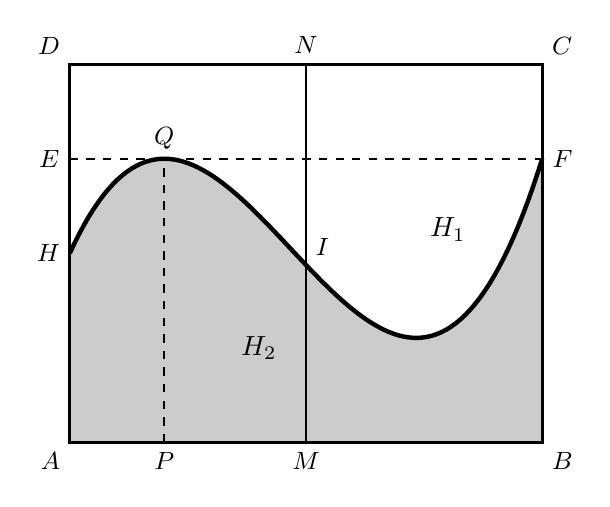
\begin{tikzpicture}[scale=0.6, >=latex]
    % 1. Tô màu vùng H2 (Người lớn) bên dưới đồ thị
    \fill[gray!40] 
        (0,0) -- (0,4) -- 
        plot[domain=0:10, samples=100] (\x, {0.05*\x*\x*\x - 0.7*\x*\x + 2.2*\x + 4}) -- 
        (10,0) -- cycle;

    % 2. Viền khung chữ nhật ABCD
    \draw[very thick] (0,0) rectangle (10,8);

    % 3. Các đường gióng đứt nét
    \draw[dashed, thick] (0,6) node[left] {\small $E$} -- (10,6) node[right] {\small $F$};
    \draw[dashed, thick] (2,0) node[below] {\small $P$} -- (2,6);
    \draw[thick] (5,0) node[below] {\small $M$} -- (5,8) node[above] {\small $N$};

    % 4. Đồ thị đường cong bậc ba
    \draw[ultra thick, domain=0:10, samples=100] 
        plot (\x, {0.05*\x*\x*\x - 0.7*\x*\x + 2.2*\x + 4});

    % 5. Tên các đỉnh và nhãn
    \node[below left] at (0,0) {\small $A$};
    \node[below right] at (10,0) {\small $B$};
    \node[above right] at (10,8) {\small $C$};
    \node[above left] at (0,8) {\small $D$};

    \node[left] at (0,4) {\small $H$};
    \node[above] at (2,6) {\small $Q$};
    \node[above right] at (5,3.75) {\small $I$};

    \node at (8,4.5) {\bfseries $H_1$};
    \node at (4,2) {\bfseries $H_2$};
\end{tikzpicture}
\end{center}
}{
    \textbf{a)} & Tọa độ của điểm \( Q \) là \( Q(2;6) \).
    & \textcolor{amberorange}{$\bigcirc$} & \textcolor{amberorange}{$\bigcirc$} \\ \hline
    
    \textbf{b)} & Phương trình của đường cong bậc ba là  
    \(f(x) = \dfrac{1}{20}x^3 + \dfrac{7}{10}x^2 + \dfrac{11}{5}x + 4.\)
    & \textcolor{amberorange}{$\bigcirc$} & \textcolor{amberorange}{$\bigcirc$} \\ \hline
    
    \textbf{c)} & Trong hệ tọa độ \( Oxy \), \( IM = \dfrac{15}{4}, IN = \dfrac{17}{4} \).
    & \textcolor{amberorange}{$\bigcirc$} & \textcolor{amberorange}{$\bigcirc$} \\ \hline
    
    \textbf{d)} & Số tiền cần bỏ ra để mắc dây đèn trang trí trên đoạn \( MN \) bằng \( 12,7 \) triệu đồng.
    & \textcolor{amberorange}{$\bigcirc$} & \textcolor{amberorange}{$\bigcirc$} \\
}

\end{document}